\chapter{The reference: purified healthy cells on the specimen's platform}\label{ch:atlas}

\section{What a reference is for}

The reference is the set of templates the chain separates a specimen into, and the standard a cell is read against. Every reading passes
through it. An error in the reference is therefore an error in every reading, and the reference has to be built with the same care as the sky
model a CMB analysis subtracts. Two rules govern what may enter. A cell enters whole or not at all: a cell measured on part of the array is
left out, because a partial cell has to be filled, and filled values are where misplaced and duplicate cells come from. And a reference is
purified healthy cells of one type; every sample, specimen or vial is a means to the methylome sought.

\section{What chain v3 reads}

Chain v3 reads five frozen reference files and nothing else. All are built from
purified EPIC v1 arrays of healthy donors~\cite{Salas2018,Salas2022}, processed from the raw IDATs by the chain's own Stage~1, so the specimen and the
reference are on one scale before anything is compared.

\begin{center}\small
\begin{tabular}{@{}p{0.33\textwidth}p{0.6\textwidth}@{}}\toprule
reference & what it holds \\\midrule
the floor & the neutrophil identity sites and the floor, 0.330263 bits \\
its held-out precision & the precision of that floor, printed with every reading \\
the residual-map reference & the sites in genome order, the healthy mean and shrunk spread of $H$ at each, and the C-score baseline \\
the composition profiles & eight blood-group profiles at the composition markers and at the neutrophil sites \\
the noise sites & the sites behind the noise index \\\bottomrule
\end{tabular}
\end{center}
\calibrated{} Every value the chain uses is read from these files by the code; none is typed. The files are named in the SOP.

\section{Counting a reference correctly}

Two public series deposit the same six physical neutrophil arrays under two accessions: each Sentrix identifier appears once in GSE110554 and once in
GSE167998. The floor file lists the six pairs it removed and counts each physical array once. \measured{} The difference matters for every check of precision. A held-out reading that keeps an array's twin in the
reference reads its own copy; counted correctly, each array read against the other five, with the identity sites re-chosen on those five, gives $A$ =
0.983--1.045 with standard deviation 0.020. \measured

Of the six reference arrays, one reads as female on its X and Y probes and five as male (Chapter~\ref{ch:skytools}). \measured{} A reference standard
states its donors' sex, and a reference of each sex is needed before a sex difference in a reading can be told from a reference effect. \openprob

\section{Why the reference must be on the specimen's platform}

A $\beta$ value depends on the chemistry and the pipeline that produced it, and the offset between two platforms is larger than the whole Normal band.
Purified neutrophils, monocytes and NK cells on 450K arrays read median 0.904--0.932 against references built on another platform, none of 8 donors in Normal; a reference from
purified 450K arrays, read leave-one-donor-out, put all eight in Normal. \measured{} Chain v3
therefore carries one reference per cell type per platform and refuses a specimen on any platform it has no reference for.

\section{Composition profiles and the person's own expectation}

The same purified arrays give the eight composition profiles. At the neutrophil identity sites the other blood cells sit close to neutrophils in
$\beta$ but not in entropy:
\begin{center}\small
\begin{tabular}{@{}lrrr@{}}\toprule
group & median $|\Delta\beta|$ from neutrophils & sites within 0.05 & mean $H$ over neutrophil mean $H$ \\\midrule
monocytes & 0.004 & 98.7~\% & 0.985 \\
eosinophils & 0.008 & 97.7~\% & 1.076 \\
basophils & 0.014 & 95.4~\% & 1.189 \\
NK cells & 0.005 & 89.9~\% & 1.151 \\
B cells & 0.016 & 79.6~\% & 1.313 \\
CD8 T cells & 0.011 & 76.9~\% & 1.326 \\
CD4 T cells & 0.019 & 75.6~\% & 1.395 \\\bottomrule
\end{tabular}
\end{center}
\calc{} from the composition profiles. Near $\beta=0.05$--0.25 and 0.75--0.95 a small difference in $\beta$ is a large
difference in $H$. A lymphocyte at a neutrophil site therefore raises the specimen's entropy there, and whole blood read against the neutrophil floor alone
reads high: six healthy DNA mixtures (neutrophils 63--75~\%) read 1.062--1.118 against the floor and 0.982--1.016 against the expectation built from their own
known composition. \measured{} The expectation, Eq.~\eqref{eq:metawb}, uses this specimen's fractions and the purified
profiles. No other person enters it.

Figure~\ref{fig:p4_profiles} shows the table site by site.

\begin{figure}[htbp]\centering
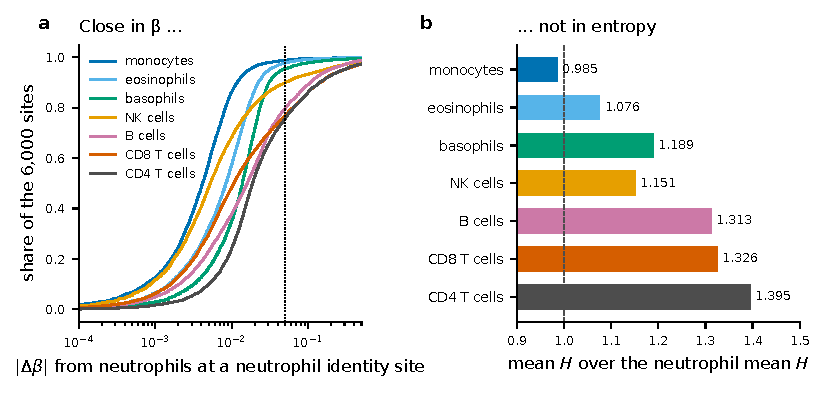
\includegraphics[width=0.95\textwidth]{figures/part6/fig_p4_14_profiles.pdf}
\caption{The other blood cells at the 6,000 neutrophil identity sites. (a) Cumulative share of sites by $|\Delta\beta|$ from the neutrophil profile;
dotted: 0.05. (b) Mean $H$ of each group over the neutrophil mean $H$. \calc{} from the
\calibrated{} profiles.}
\label{fig:p4_profiles}
\end{figure}

The composition profiles are built from both Salas series, which share the six neutrophil arrays. The known mixtures of the acceptance run come from one of
those series, so the profiles and the mixtures are not independent there; the independent test used profiles from the other study only. \measured

\section{The multi-source atlas}

A posterior atlas assembled from many sources and platforms is held in the repository.
Chain v3 does not read it. Whether it enters the chain, and on what scale, is decided cell type by cell type as each is commissioned. \openprob

\section{What the reference does not yet do}

It holds one cell type with identity sites and a floor (neutrophils, EPIC v1). It rests on six physical arrays from one laboratory, five male and one
female. It has no 450K or EPIC v2 version in the chain. Floors for other cell types exist for development only and are not read. Each further cell type enters only after it passes three tests:
held-out precision of its own floor, recovery in known mixtures, and a known change read in the right direction (the SOP). \openprob

\section{Atlas v2: the reference for the cells that come next}

The neutrophil reference and the eight composition profiles of chain v3 come from purified EPIC arrays, as above. Atlas v2
is the reference from which the identity sites and profiles of each further cell type will be drawn as that type is commissioned. It was built
to the same rule: every cell type measured on purified healthy cells of that type, nothing filled, every value with its uncertainty.

\section{The model}

The second atlas is one hierarchical fit. For locus $i$, cell $c$ and source $s$ (one published data set on one platform),
\begin{align}
  \beta^{\mathrm{obs}}_{ics}&\sim\mathcal N\!\left(\mu_{ic}+\delta_{is},\ \sigma^2_{\mathrm{obs},s}+\sigma^2_{\mathrm{loc},i}\right)\quad\text{where measured},\\
  \mu_{ic}&=m_i+e_{ic},\qquad e_{ic}\sim\mathcal N(0,\tau^2),
\end{align}
with $m_i$ the locus's shared level and $\delta_{is}$ the source term: what one laboratory's platform and pipeline add to every cell it
measured. The inputs are the \emph{samples} behind each published table, at every locus they measured, so the model sees real donor-to-donor
spread. Nothing in it reads a patient, a specimen or a laboratory of patients; the floors are not refitted. No grouping of cells into classes enters
the fit: each cell's mean is pulled toward the locus's shared level only, so no cell is drawn toward the mean of a group it
belongs to. Two consequences follow by construction.
\begin{enumerate}
\item The same cell from two sources shares one $\mu_{ic}$ and differs only by $\delta$: twins become one cell.
\item Where a cell's sources never measured a locus, $\mu_{ic}$ is left \emph{blank}, not filled. The number of observations behind every value,
      $n_{\mathrm{obs}}$, is stored beside it.
\end{enumerate}

\section{Sources and the entry rule}

\begin{center}\small
\begin{tabularx}{\linewidth}{@{}>{\raggedright\arraybackslash}X>{\raggedright\arraybackslash}X>{\raggedright\arraybackslash}X@{}}\toprule
source & form & entered as \\\midrule
Moss 2018~\cite{Moss2018} (GSE122126) & raw 450K/EPIC IDATs & through the chain's own Stage~1 \\
Salas 2018, 2022~\cite{Salas2018,Salas2022} (GSE110554, GSE167998) & raw IDATs of sorted blood & through Stage~1 \\
GSE63409 & raw IDATs of sorted HSC and progenitors & through Stage~1 \\
Loyfer 2023~\cite{Loyfer2023} (GSE186458) & WGBS $\beta$ and depth at array CpGs & per-locus, $\ge10$ reads \\
Tian 2023~\cite{Tian2023} (GSE215353) & brain single-cell pseudobulk & pooled; flagged \\
ENCODE & WGBS of tissues and embryonic stem lines & per-locus, $\ge10$ reads \\\bottomrule
\end{tabularx}
\end{center}
A cell enters only if it has at least two independent donors; every array passes intake and every sequencing sample has at least ten reads at
90~\% of loci; it is not a twin of an existing cell; and it reads 1.00 on its own profile. A cell failing any of these waits for data. The twin
test was made at the level of samples: a CpG counts as separating two cells only when every sample of one lies more than 0.20 beyond every sample of
the other. Sampling noise cannot manufacture that. By it, a kidney podocyte entry was found to be sorting impurity from tubule (no
hypomethylation at the podocyte genes \emph{NPHS1}, \emph{PODXL}, \emph{WT1}), and mixtures were removed. Seventy-four cells entered.
Because a reference is one purified cell type, profiles of whole tissues are test specimens for the atlas, not references in it.

\section{Putting sequencing on the array scale}

The atlas sits on the chain's own array scale. Sequencing sources enter through their source terms, estimated in closed form: for each sequencing
source, a Deming regression of its per-locus cell means on the array means of the same cells, over 50,000 loci, with a bootstrap over cells. A first
cross-platform measurement on ten cell types measured both ways gave slopes of 1.03--1.09 and intercepts of $-0.04$ to $-0.07$ for every cell type:
one transfer between platforms, not a per-cell difference. \measured{} Two sources share no cell with any other and their terms cannot be measured:
the stem-line sequencing, which was later bridged by an embryonic-stem-cell array series with raw IDATs (GSE116754), and GSE63409's sorted
progenitors, which take an array offset of zero. Both are kept in and labeled for what they are: the progenitor source term
is carried with status ASSUMED and an estimated effect on $A$ of at most about 0.015, and every reading on those cells carries the flag.

\section{The fit}

A source's terms trade off against the means of every cell only it measured, so the source terms are fixed from the closed form. A test block of about 1,000 loci converged
($\hat R$ 99th percentile 1.005, effective sample size 1st percentile 753, no divergences), at 0.83~s per locus. The full fit then ran over about
814,000 loci in 700 blocks with NUTS~\cite{Hoffman2014} in NumPyro, on rented cloud machines, every finished block copied to storage as it landed.
Twenty posterior draws per cell per locus were kept. A whole-atlas gate confirmed that no two cells came out identical and that no value was filled
where a cell was unmeasured; 0.19~\% of values were flagged for per-block convergence and kept with the flag. \measured

\section{Does the atlas tell the truth about itself?}

A posterior interval is only useful if it covers the truth at the stated rate. A pre-registered held-out check hid 5~\% of the observations in 20 randomly chosen blocks, refitted
those blocks, and asked how often the held-out values fell inside the atlas's 90~\% predictive interval (Figure~\ref{fig:v5}). \measured

\begin{figure}[htbp]\centering
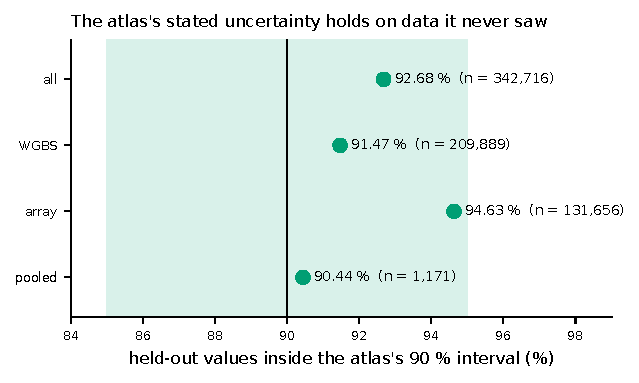
\includegraphics[width=0.75\textwidth]{figures/part6/fig_v5.pdf}
\caption{Coverage of held-out observations by the atlas v2 90~\% interval, overall and by kind of data; shaded band is the pre-registered pass range,
85--95~\%. 342,716 held-out observations in 20 blocks; every block 92.3--93.1~\%; no divergences. \measured}
\label{fig:v5}
\end{figure}

The atlas's stated uncertainty is honest and slightly conservative: 92.7~\% against a nominal 90~\%. The lowest cells were smooth muscle (82.9~\%) and
aorta and lung alveolar endothelium (about 89~\%); the highest were three bone-marrow progenitors (CMP, L-MPP, MPP) and kidney glomerular
epithelium, at 96.9--97.2~\%. Mean absolute prediction error was 0.051. \measured

\paragraph{What a posterior interval is not.} The posterior standard deviation of an atlas value says how well the data pin down
the healthy mean of one cell type at one site. It is not the spread of healthy cells about that mean. For a value built from $n$
independent samples the first is about $\sqrt n$ times smaller than the second: six times for $n=36$. \derived{} A healthy range
built as the mean $\pm1.96$ posterior standard deviations is therefore a category error: the precision of an average used as the
width of a distribution, which places ordinary healthy specimens many standard deviations outside it. No reading in this book uses
a posterior interval as a range. Two intervals are kept apart instead: the precision of the reference itself (for neutrophils on
EPIC, the held-out standard deviation 0.020, Chapter~\ref{ch:meta}) and the specimen's own detection limit
(Chapter~\ref{ch:instrument}). Neither is a range of people; healthy is $A=1$.


\section{What is in it}

Seventy-four cell types. Cells the first atlas named but the second does not contain are not lost; they wait for data that meet
the entry rule. The candidates for the next additions are further cell types measured on the whole array or by whole-genome sequencing of purified
cells, entered one at a time through the same script and the same checks.

\section{What this atlas does that a reference panel does not}

Methylation references in common use are tables: one number per CpG per cell type, at a few hundred to a few thousand marker CpGs chosen
because they separate cell types, each table built on its own laboratory's arrays and pipeline. They are built to answer one question: how
much of each cell is in this specimen. The atlas here was built to answer a second one as well, how well each cell is holding its own pattern,
and that question puts requirements on a reference that a marker table does not meet.
\begin{center}\small
\begin{tabular}{@{}p{0.27\textwidth}p{0.3\textwidth}p{0.35\textwidth}@{}}\toprule
property & a marker reference table & atlas v2 \\\midrule
what is stored per CpG per cell & one mean & posterior mean, SD, 95\,\% interval, 20 posterior draws, and $n_{\rm obs}$ \\
how many CpGs & a marker panel & about 814,000, every array CpG with data \\
how sure each value is & not stated & stated, and checked: held-out coverage 92.7\,\% against 90\,\% nominal \\
laboratory and pipeline effects & built into the means & a separate source term $\delta_{is}$, so the cell's own level is not one laboratory's \\
scale & the publishing group's pipeline & the chain's own Stage~1, the same calibration a patient's array goes through \\
the same cell from two sources & two entries, solved apart & one cell by construction \\
a CpG never measured in a cell & often filled with an average & left blank; nothing is filled \\
entry & any published profile & at least two donors, a sample-level twin test, and the cell reads 1.00 on its own profile \\\bottomrule
\end{tabular}
\end{center}

What that buys, in order of consequence:
\begin{enumerate}
\item \textbf{A reading per person, not a position in a group.} The atlas is a reference for each cell type, measured on purified healthy
cells of that type. A specimen is read against it and against nothing else: no other patient, no group mean, no percentile. The test the report
applies to every number it prints is whether that number could exist if nobody else's specimen had ever been measured; every reading passes it.
\item \textbf{The reference says how far it can be trusted.} Because every value carries its posterior, a cell whose reference is well measured
gives a tight reading and a poorly measured one gives a wide one, and the reader is told which. The atlas's stated intervals were tested on
observations it had not seen and covered them at the stated rate. \measured
\item \textbf{The reference can be read on the patient's scale.} A $\beta$ value depends on the pipeline that produced it, and the offset
between two pipelines is larger than the whole Normal band. The atlas sits on the chain's own Stage~1 scale, and sequencing sources enter
through measured source terms, so a patient's array and the reference are on one scale before anything is compared. \measured
\item \textbf{Composition and fidelity from one reference.} The same posterior means can both separate a specimen into its cells and define each
cell's identity sites; chain v3 does this for blood from the purified EPIC profiles. In whole blood the expectation is built from the person's own composition: six healthy DNA mixtures of known composition (neutrophils
63--75\,\%) read 1.062--1.118 against the neutrophil reference alone and 0.982--1.016 against their own composition. \measured
\item \textbf{It knows what it cannot do.} Pairs of cells the arrays cannot tell apart are named as such rather than given a split; cells whose
data do not meet the entry rule are absent rather than approximated; every
value carries the number of observations behind it.
\item \textbf{Every number can be rebuilt.} Every step is a numbered script with fixed random seeds, every source is public, and every block
of the fit is stored with its SHA-256, so a rebuild on the same package versions reproduces the posterior draws, not only the means.
\end{enumerate}

What it does not yet do, stated so that no reader assumes it: it holds 74 cell types, not every cell in the body; it does not store the
covariance between cell types at a site, so two cells that trade off against each other are each reported with their own uncertainty and
not with the tighter uncertainty of their sum; the progenitor source term is assumed rather than measured; and chain v3 does not read it yet. \openprob
